\documentclass{article}
\usepackage[utf8]{inputenc}
\usepackage{amsmath, dsfont, mathtools}
\usepackage{graphicx, float}
\usepackage[most]{tcolorbox}
\usepackage{enumitem}
\usepackage{hyperref}
\usepackage{tikz}
\usepackage{circuitikz}
\usetikzlibrary{calc}
\usepackage{xcolor}

% ------------------------------------ %
%             Customization            %
% ------------------------------------ %

\usepackage[letterpaper, top=1in, left=1in, right=1in, bottom=1in]{geometry}
\setlength{\parindent}{0em}
\setlength{\parskip}{0.5em}
\setlist[enumerate]{itemsep=-0.5em} % Adjust the spacing as desired
\setlist[itemize]{itemsep=-0.5em} % Adjust the spacing as desired
\renewcommand{\baselinestretch}{1.25}

\title{MATH1853}
\author{Jax T}
\date{23 Dec}

\newtcolorbox{knBox}[2][]{
arc=2mm, 
lower separated=true, % Set to true to enable the separation between upper and lower sections
segmentation style={dashed, draw=black}, % Add dashed line style between the sections
fonttitle=\bfseries,
colbacktitle=white!10,
coltitle=black,
enhanced,
attach boxed title to top left={xshift=0.2cm,
        yshift=-2mm},
colframe=white!40!black,
boxrule=0.3mm,
colback=black!02,
title=#2,#1
}

\newtcolorbox{definition}[2][]{
arc=2mm, 
lower separated=true, % Set to true to enable the separation between upper and lower sections
segmentation style={dashed, draw=black}, % Add dashed line style between the sections
fonttitle=\bfseries,
colbacktitle=green!10,
coltitle=black,
enhanced,
attach boxed title to top left={xshift=0.2cm,
        yshift=-2mm},
colframe=green!40!black,
boxrule=0.3mm,
colback=green!02,
title=#2,#1
}

\hypersetup{
    colorlinks=true,
    linkcolor=purple    % Color for internal links
}

\newenvironment{amatrix}[1]{%
  \left[\begin{array}{@{}*{#1}{c}|c@{}}
}{%
  \end{array}\right]
}

\newcommand{\note}[1]{\textcolor{gray}{\tiny #1}}

% ------------------------------------ %
%              Title page              %
% ------------------------------------ %
\begin{document}

\begin{titlepage}
    \null\vfill % Add vertical space to center the title and author
    
    \centering
    \Huge\textbf{ENGG1300}
    
    \vspace{0.1cm}
    \Large\textbf{Notes Spring 2024}
    
    \vspace{1cm}
    \normalsize\textbf{Author:} Jax
    
    \normalsize\textbf{Contact:} enhanjax@connect.hku.hk
    \vfill % Add vertical space to center the remaining space
\end{titlepage}

% ------------------------------------ %
%               Document               %
% ------------------------------------ %

\section{Vectors}

\begin{definition}[]{Basics}
  Vector can be represented by $\vec{F}$ or $\boldsymbol{F}$. The magnitude can be represented by $|F|$ or $F$.
\end{definition}

\begin{definition}[]{Parallelogram law}

  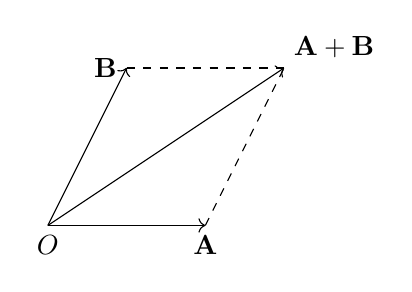
\begin{tikzpicture}
    % Define the coordinates
    \coordinate (O) at (0,0);
    \coordinate (A) at (2,0);
    \coordinate (B) at (1,2);
    \coordinate (C) at ($(A)+(B)$);
    
    % Draw the vectors
    \draw[->] (O) -- (A);
    \draw[->] (O) -- (B);
    \draw[->] (O) -- (C);
    
    % Draw the parallelogram
    \draw[dashed] (A) -- (C);
    \draw[dashed] (B) -- (C);
    
    % Label the vectors and points
    \node[below] at (O) {$O$};
    \node[below] at (A) {$\mathbf{A}$};
    \node[left] at (B) {$\mathbf{B}$};
    \node[above right] at (C) {$\mathbf{A} + \mathbf{B}$};
  \end{tikzpicture}

  $C=A+B=\sqrt{A^2+B^2-2AB\cos{\gamma}},\quad\text{where }\gamma=\angle OAC$
  
\end{definition}

\begin{knBox}[]{Unit vectors}
  They are vectors with magnitude 1. $\hat{A}=\frac{\vec{A}}{|\vec{A}|}$
\end{knBox}

\subsection{Coplanar vectors}
\begin{definition}
  {Cartesian vector notation}

  In two dimensions, the Cartesian unit vectors $\boldsymbol{i}, \boldsymbol{j}$ are used to designate the directions of the x and y axes respectively.

  $F=F_x \boldsymbol{i} + F_y \boldsymbol{j},\quad\text{where }F_{x/y}$ is the $x/y$ component of $F$
\end{definition}

\begin{knBox}
  {Resultant force}
  The resultant force $F_R$ can be found by the sum of the components of $F$: $F_R=F_1+F_2=(F_{x1}+F_{x2})\boldsymbol{i}+(F_{y1}+F_{y2})\boldsymbol{j}$
\end{knBox}
\begin{knBox}
  {Orientation of vector}
  We always consider the angle between $F$ \& $F_x$. It can be found by $\theta=\tan^{-1}\frac{F_y}{F_x}$.
\end{knBox}
\begin{knBox}
  {Magnitude of forces}
  Magnitude: $|F|=\sqrt{F_x^2+F_y^2}$

  Magnitude of $x$ component: $F_x=F\sin{\theta}$

  Magnitude of $y$ component: $F_y=F\cos{\theta}$
\end{knBox}
\subsection{Vectors in 3D}
The concepts above can be extended to 3D simply by adding another variable to the system.
\begin{knBox}
  {Coordinate direction angles in 3D}
  The direction of A is defined by the \emph{coordinate direction angles}: $\alpha, \beta, \gamma$, which are measured between the tail of A and the positive $x, y, z$ axes. 
  \[\alpha=\cos^{-1}\frac{A_x}{A},\quad\beta=\cos^{-1}\frac{A_y}{A},\quad\gamma=\cos^{-1}\frac{A_z}{A}\]
  \begin{center}
    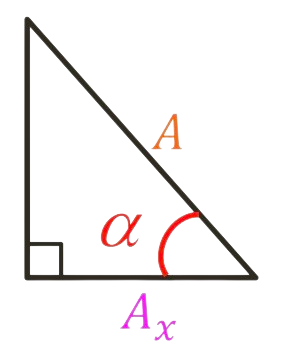
\includegraphics[width=2cm]{img/Ax.png}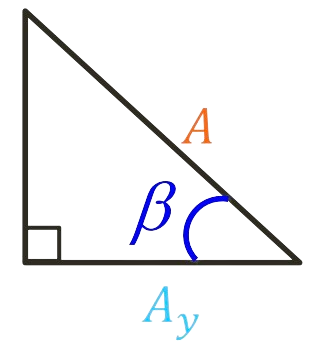
\includegraphics[width=2cm]{img/Ay.png}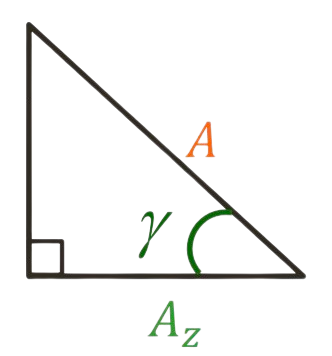
\includegraphics[width=2cm]{img/Az.png}
  \end{center}
\end{knBox}

\subsection{Vectors along a line}
We can formulate a force $F$ along a line as a Cartesian vector using unit vectors along the axes. Note that the unit vectors can easily be expressed as Cartesian. 
\begin{definition}
  {Formulating vectors by unit vectors}
  $\vec{F}=|F|\times\hat{F}=|F|\times\frac{r}{|r|}$
\end{definition}
\subsubsection{Simple example}
\begin{center}
  Consider the following graph:
  
  \begin{figure}[!ht]
    \centering
    \resizebox{0.2\textwidth}{!}{%
    \begin{circuitikz}
    \tikzstyle{every node}=[font=\normalsize]
    \node [font=\normalsize] at (10.5,10) {F = 100N};
    \draw [->, >=Stealth] (8.25,11) .. controls (9.75,9.75) and (9.75,9.75) .. (11,8.5);
    \draw [dashed] (8.25,11) .. controls (8.25,9.75) and (8.25,9.75) .. (8.25,8.5);
    \draw [dashed] (8.25,8.5) .. controls (9.75,8.5) and (9.75,8.5) .. (11,8.5);
    \node [font=\normalsize] at (7.75,9.5) {4};
    \node [font=\normalsize] at (9.5,8) {4};
    \node [font=\normalsize] at (8.25,11.25) {A};
    \node [font=\normalsize] at (11.25,8.25) {B};
    \end{circuitikz}
    }%
    \label{fig:my_label}
  \end{figure}
  
  First, we consider $r_{AB}$. From the graph:
  \[\vec{r_{AB}}=4\boldsymbol{i}+4\boldsymbol{j}\]
  Then, we find the magnitude of $r_{AB}$:
  \[|r_{AB}|=\sqrt{4^2+4^2}=5.65\dots\]
  Finally, we apply our formula for $F$:
  \begin{align*}
    \vec{F}=|F|\times\frac{r_{AB}}{|r_{AB}|}&=100\times(\frac{r_x}{5.65}\boldsymbol{i}+\frac{r_y}{5.65}\boldsymbol{j})\\&=100\times(\frac{4}{5.65}\boldsymbol{i}+\frac{4}{5.65}\boldsymbol{j})\\&=70.7\boldsymbol{i}+70.7\boldsymbol{j}N
  \end{align*}
\end{center}

\section{Cross products}
The cross product of $A\times B$ gives a new vector $C$.
\begin{definition}
  {Finding the cross product via Cartesian vectors}
  \[A\times B=\begin{vmatrix}
    i&j&k\\
    A_x&A_y&A_z\\
    B_x&B_y&B_z
  \end{vmatrix}=C\]
\end{definition}
\begin{definition}
  {Magnitude of cross product}
  \[|C|=|A||B|\sin\theta\]
\end{definition}

\section{Moment of forces}
\begin{definition}
  {Definition of moment}
  The moment of a force is a measure of its \emph{tendency} to cause a body to rotate about a specific point.

  The moment about a point $O$, when $F$ is applied a distance $d$ from the point is: 
  \[M_O=F\times d\]
  Keep in mind that \emph{positive} moment is \emph{anti-clockwise}.
\end{definition}
\begin{knBox}
  {Resultant moments}
  The resultant moment is the \textbf{sum} of all moments present on the point.
\end{knBox}
\subsection{Coplanar moments}
\subsubsection{Finding the moment of a non-linearly attached force}
One simple way is to find the \emph{components} of the force, and sum their individual moments together. The following is a simple example:
\begin{center}
  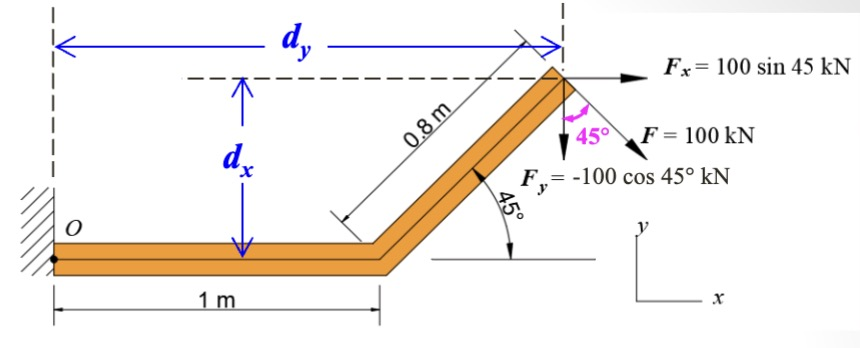
\includegraphics[width=10cm]{img/Moment1.jpg}
  
  After finding the component forces of $F$, we can deduce the resultant moment to be:
  \begin{align*}
    M_O&=F_x\times 0.8\sin 45\deg+F_y\times(1+0.8\cos 45\deg)\\
    &=-150.7kNm
  \end{align*}
\end{center}

\subsection{Non-coplanar moments}
\begin{definition}
  {Moment formulation by cross products}
  Consider $\vec{r}$ a position vector drawn from $O$ to any point on the \emph{line of action} of $F$. The moment can hence be given by:
  \[M_O=r\times F\]
  \begin{center}
    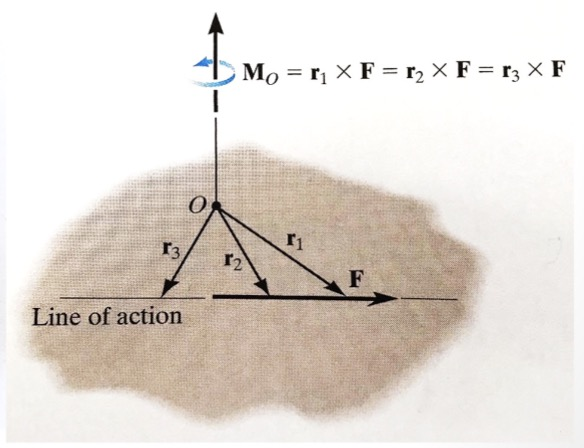
\includegraphics[width=0.4\textwidth]{img/Moment2.jpg}
  \end{center}
\end{definition}

\subsection{Couple moments}


\end{document}